\section{Erzeugung der Eingangsbilder}

Die Erzeugung von Eingangsbildern für unser neuronales Netz, war eines der ersten Probleme, welches wir gelöst haben. Testbilder zu suchen oder selbst zu erstellen kann sehr zeitaufwendig sein. Aus diesem Grund haben wir zwei Matlab-Skripte geschrieben, die uns dieses Problem zukünftig abnehmen. Die beiden Dateien heißen 'GetPixelFeatureMatrix.m' \ref{GetPixelFeatureMatrix} und 'GetInputFeatureMatrix.m' \ref{GetInputFeatureMatrix}. Die Funktion 'GetPixelFeatureMatrix' erwartet als Eingang eine Merkmale-Matrix, die dann auf eine Pixel-Matrix hochskaliert wird. Darüber hinaus kann auch ein Rauschwert angegeben werden, um das neuronale Netz auf Rauschempfindlichkeit zu testen. Im Anschluss sind ein paar Bilder erzeugt worden. Im Sinne der Lesbarkeit sind im Weiteren alle angebenen Werte für Merkmale, Pixel oder Pixel pro Merkmal lediglich für eine Dimension angegeben, da diese stets symmetrisch sind. Die ersten beiden Abbildungen sollen die Flexibilität der Funktion verdeutlichen und verfügen über 7 Merkmale, 64 Pixel pro Merkmal und einen Rauschanteil von 10\%. Die meisten der nachfolgenden Abbildungen verfügen über fünf Merkmale, 128 Pixel pro Merkmal und somit insgesamt über 640 Pixel und unterscheiden sich neben des dargestellten Musters hauptsächlich in ihrer Rauschintensität. Eine Ausnahme bildet lediglich die Abbildung \ref*{585px9M65pM10} mit 9 Merkmalen, 65 Pixeln pro Merkmal und einem Rauschanteil von 10\%. Somit wird bei den Bildern lediglich die Besonderheiten beziehungsweise der jeweilige Rauschanteil genannt.

\begin{figure}[hbt]
	\begin{minipage}{0.49 \textwidth}
		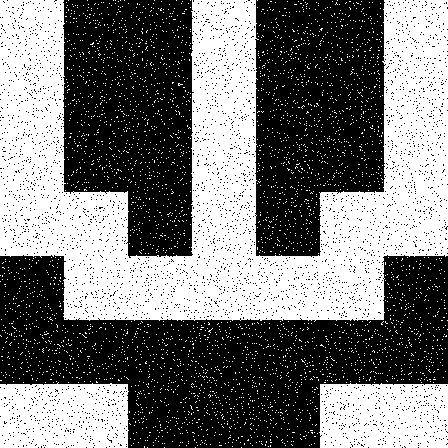
\includegraphics[width=\textwidth]{./Bilder/Auswertung/BeispielBilder/Picture_Example4_noise_10_pixelCnt_64_featureCnt_7}
		\caption{Beispielbild 1 mit 10\% Rauschen}
		\label{Toni_Avatar}
	\end{minipage}
	\hfill
	\begin{minipage}{0.49 \textwidth}
		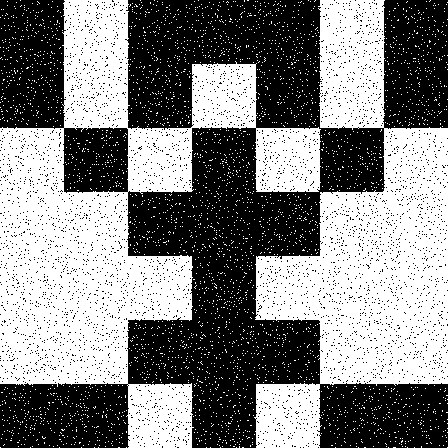
\includegraphics[width=\textwidth]{./Bilder/Auswertung/BeispielBilder/Picture_Example2_noise_10_pixelCnt_64_featureCnt_7}
		\caption{Beispielbild 2 mit 10\% Rauschen}
		\label{Bryan_Avatar}
	\end{minipage}
\end{figure}

\begin{figure}[hbt]
	\begin{minipage}{0.49 \textwidth}
		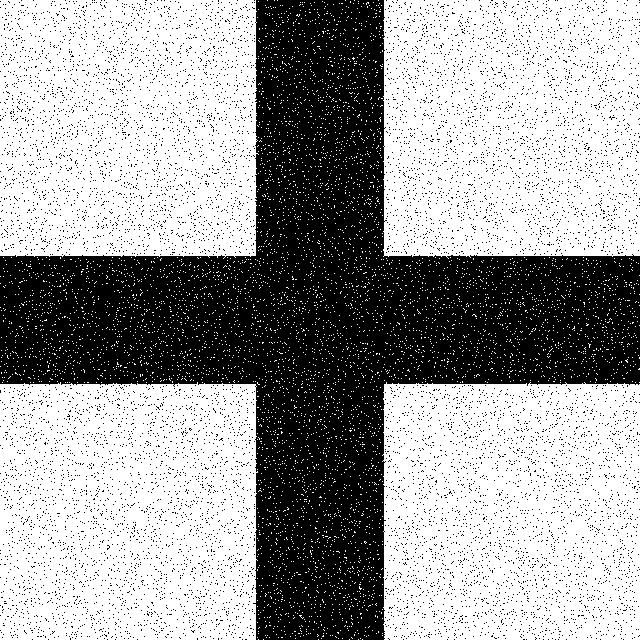
\includegraphics[width=\textwidth]{./Bilder/Auswertung/BeispielBilder/Picture_Crossing_noise_10_pixelCnt_128_featureCnt_5}
		\caption{Kreuz mit 10\% Rauschen}
		% \label{eindeutigerBezeichner}
	\end{minipage}
	\hfill
	\begin{minipage}{0.49 \textwidth}
		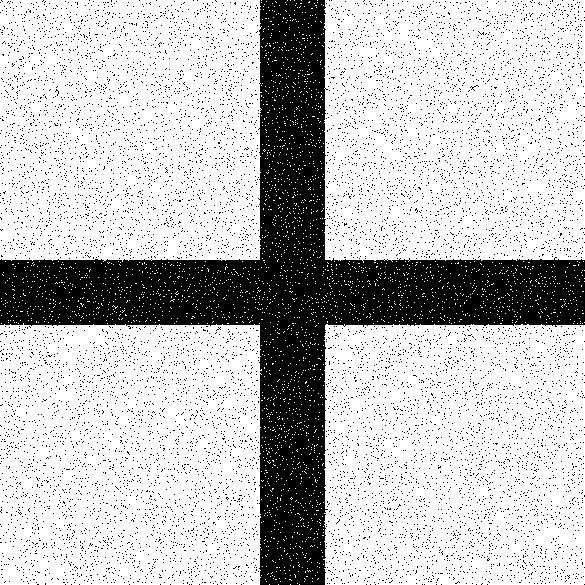
\includegraphics[width=\textwidth]{./Bilder/Auswertung/BeispielBilder/Picture_Crossing_noise_10_pixelCnt_65_featureCnt_9}
		\caption{9 Merkmale \& 10\% Rauschen}
		\label{585px9M65pM10}
	\end{minipage}
\end{figure}

\begin{figure}[hbt]
	\begin{minipage}{0.49 \textwidth}
		
\includegraphics[width=\textwidth]{./Bilder/Auswertung/BeispielBilder/Picture_Line1_noise_10_pixelCnt_128_featureCnt_5}
		\caption{Horizontal mit 10\% Rauschen}
		% \label{eindeutigerBezeichner}
	\end{minipage}
	\hfill
	\begin{minipage}{0.49 \textwidth}
		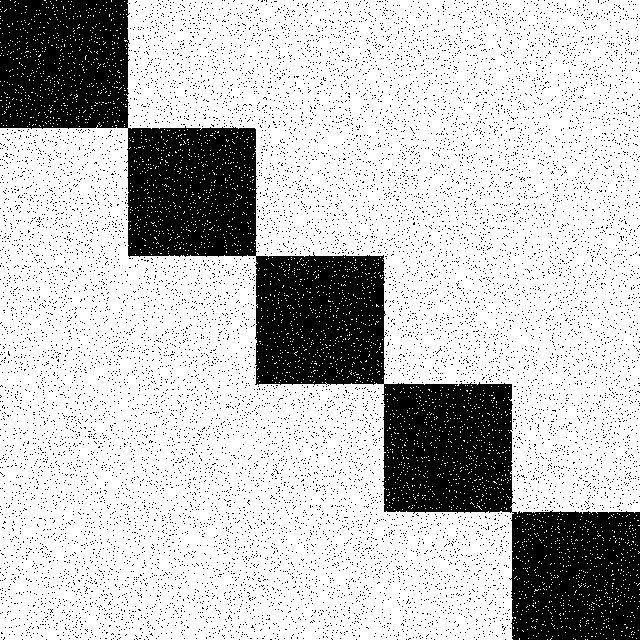
\includegraphics[width=\textwidth]{./Bilder/Auswertung/BeispielBilder/Picture_Line2_noise_10_pixelCnt_128_featureCnt_5}
		\caption{Diagonale mit 10\% Rauschen}
		% \label{eindeutigerBezeichner}
	\end{minipage}
\end{figure}

\begin{figure}[hbt]
	\begin{minipage}{0.49 \textwidth}
		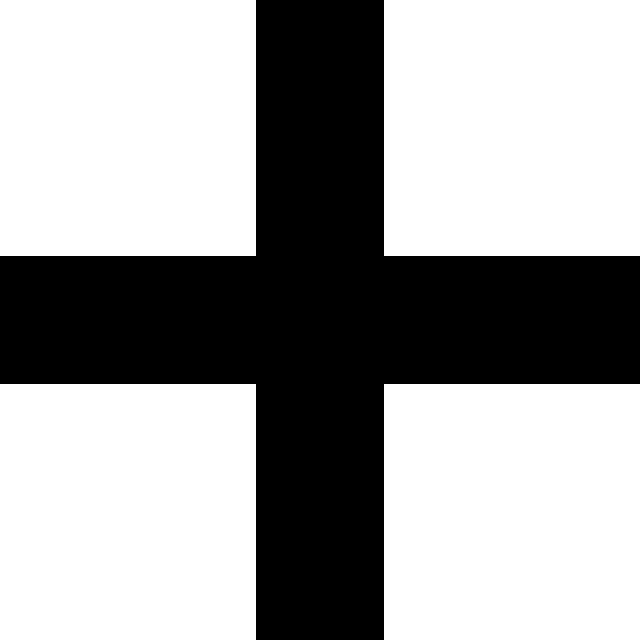
\includegraphics[width=\textwidth]{./Bilder/Auswertung/BeispielBilder/Picture_Crossing_noise_0_pixelCnt_128_featureCnt_5}
		\caption{Kreuz ohne Rauschen}
		% \label{eindeutigerBezeichner}
	\end{minipage}
	\hfill
	\begin{minipage}{0.49 \textwidth}
		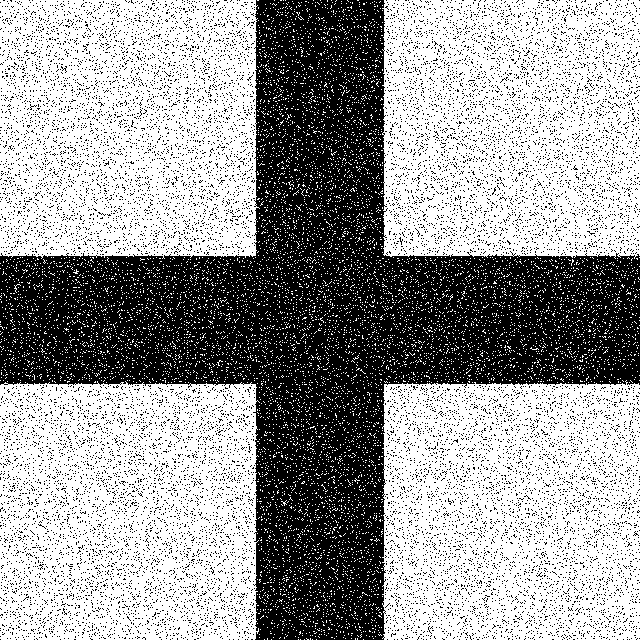
\includegraphics[width=\textwidth]{./Bilder/Auswertung/BeispielBilder/Picture_Crossing_noise_20_pixelCnt_128_featureCnt_5}
		\caption{Kreuz mit 20\% Rauschen}
		% \label{eindeutigerBezeichner}
	\end{minipage}
\end{figure}

\begin{figure}[hbt]
	\begin{minipage}{0.49 \textwidth}
		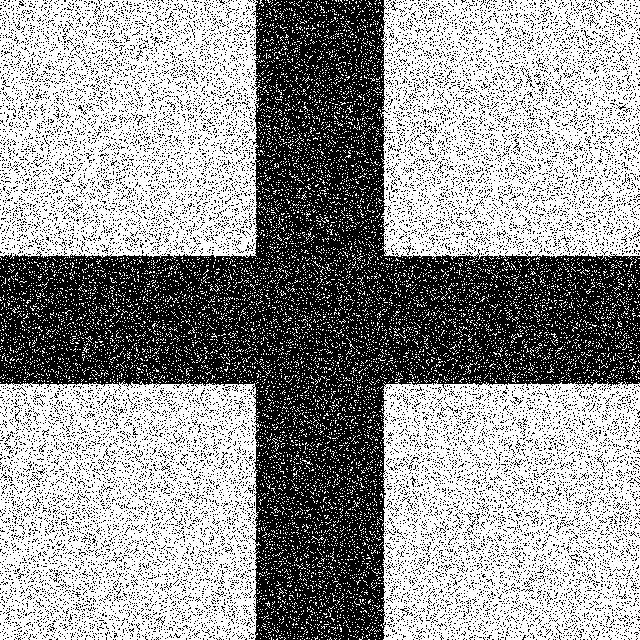
\includegraphics[width=\textwidth]{./Bilder/Auswertung/BeispielBilder/Picture_Crossing_noise_30_pixelCnt_128_featureCnt_5}
		\caption{Kreuz mit 30\% Rauschen}
		% \label{eindeutigerBezeichner}
	\end{minipage}
	\hfill
	\begin{minipage}{0.49 \textwidth}
		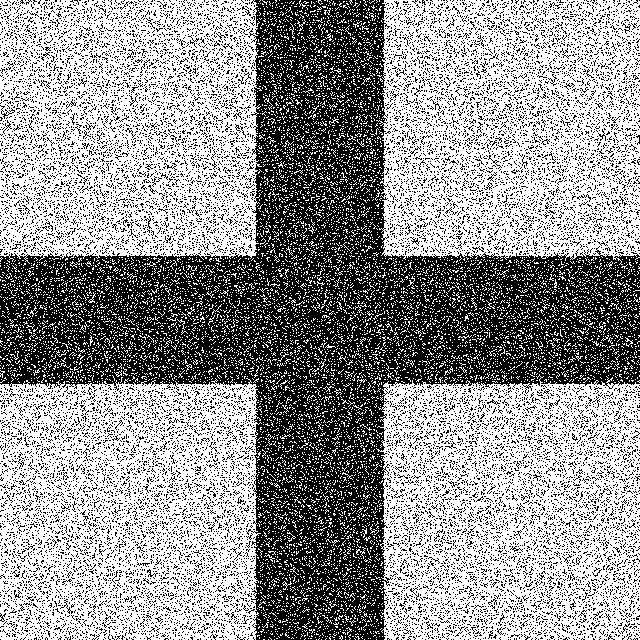
\includegraphics[width=\textwidth]{./Bilder/Auswertung/BeispielBilder/Picture_Crossing_noise_40_pixelCnt_128_featureCnt_5}
		\caption{Kreuz mit 40\% Rauschen}
		% \label{eindeutigerBezeichner}
	\end{minipage}
\end{figure}

\begin{figure}[hbt]
	\begin{minipage}{0.49 \textwidth}
		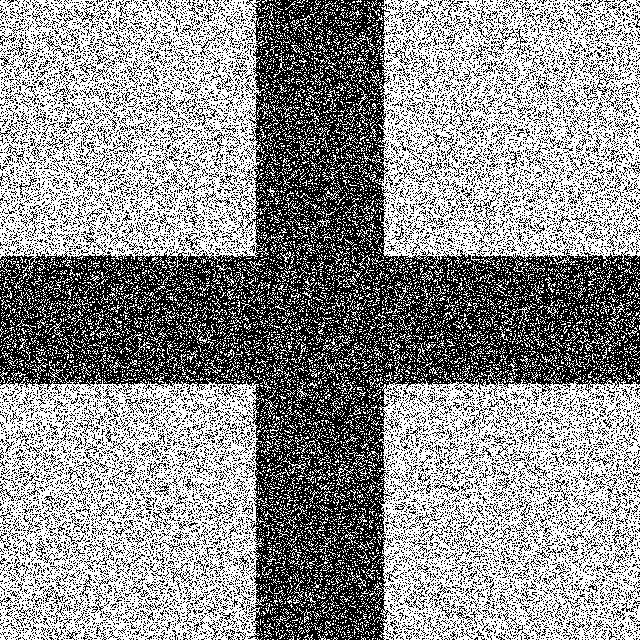
\includegraphics[width=\textwidth]{./Bilder/Auswertung/BeispielBilder/Picture_Crossing_noise_50_pixelCnt_128_featureCnt_5}
		\caption{Kreuz mit 50\% Rauschen}
		% \label{eindeutigerBezeichner}
	\end{minipage}
	\hfill
	\begin{minipage}{0.49 \textwidth}
		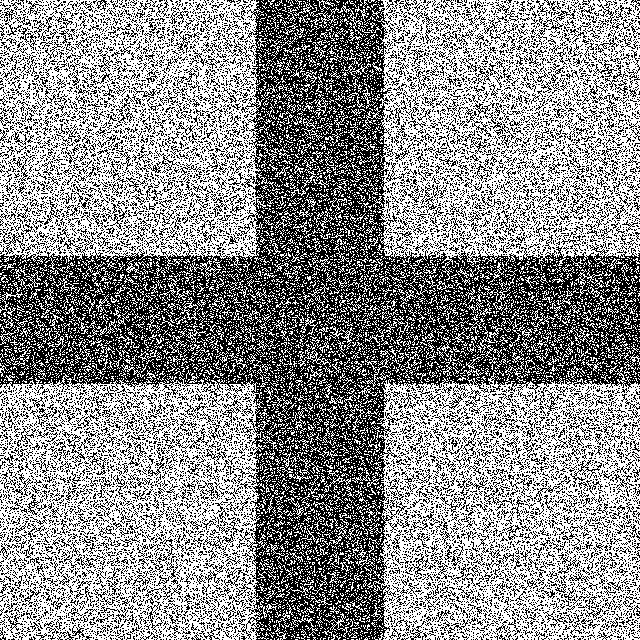
\includegraphics[width=\textwidth]{./Bilder/Auswertung/BeispielBilder/Picture_Crossing_noise_60_pixelCnt_128_featureCnt_5}
		\caption{Kreuz mit 60\% Rauschen}
		% \label{eindeutigerBezeichner}
	\end{minipage}
\end{figure}

\begin{figure}[hbt]
	\begin{minipage}{0.49 \textwidth}
		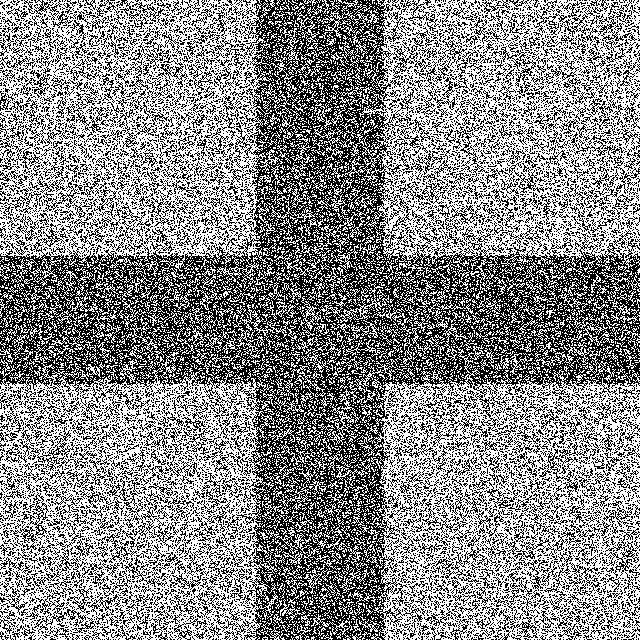
\includegraphics[width=\textwidth]{./Bilder/Auswertung/BeispielBilder/Picture_Crossing_noise_70_pixelCnt_128_featureCnt_5}
		\caption{Kreuz mit 70\% Rauschen}
		% \label{eindeutigerBezeichner}
	\end{minipage}
	\hfill
	\begin{minipage}{0.49 \textwidth}
		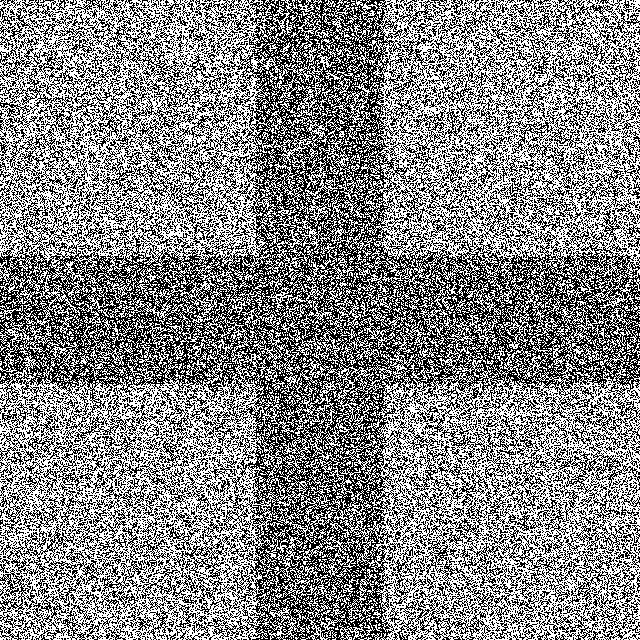
\includegraphics[width=\textwidth]{./Bilder/Auswertung/BeispielBilder/Picture_Crossing_noise_80_pixelCnt_128_featureCnt_5}
		\caption{Kreuz mit 80\% Rauschen}
		% \label{eindeutigerBezeichner}
	\end{minipage}
\end{figure}

\begin{figure}[hbt]
	\begin{minipage}{0.49 \textwidth}
		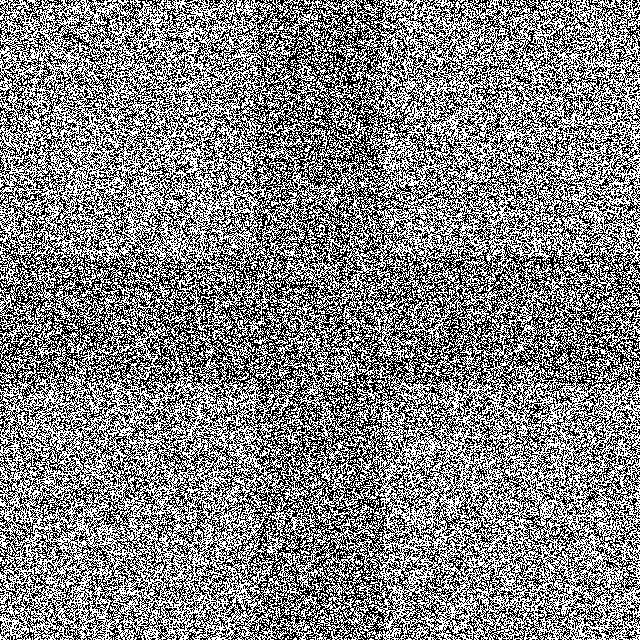
\includegraphics[width=\textwidth]{./Bilder/Auswertung/BeispielBilder/Picture_Crossing_noise_90_pixelCnt_128_featureCnt_5}
		\caption{Kreuz mit 90\% Rauschen}
		% \label{eindeutigerBezeichner}
	\end{minipage}
	\hfill
	\begin{minipage}{0.49 \textwidth}
		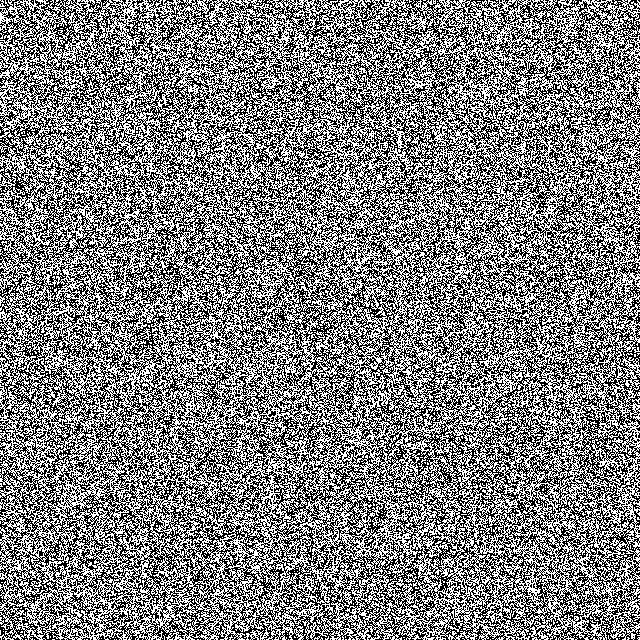
\includegraphics[width=\textwidth]{./Bilder/Auswertung/BeispielBilder/Picture_Crossing_noise_100_pixelCnt_128_featureCnt_5}
		\caption{Kreuz mit 100\% Rauschen}
		% \label{eindeutigerBezeichner}
	\end{minipage}
\end{figure}

\begin{figure}[hbt]
	\centering
	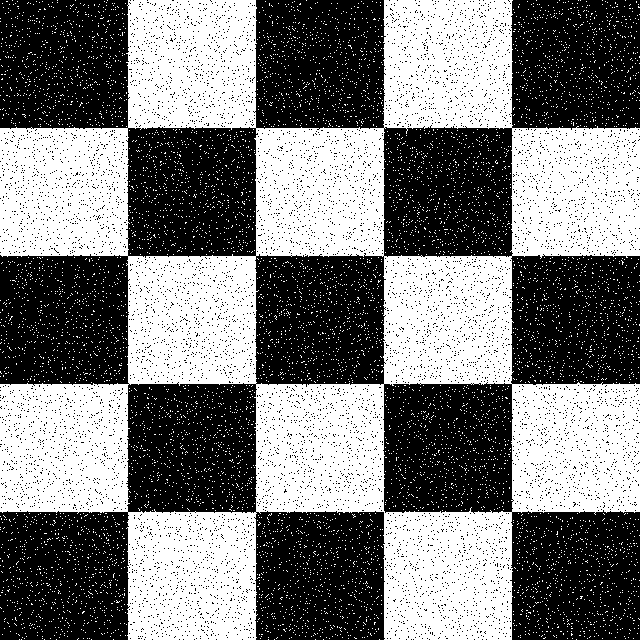
\includegraphics[width=0.7\linewidth]{./Bilder/Auswertung/BeispielBilder/Picture_Example1_noise_10_pixelCnt_128_featureCnt_5}
	\caption{Schachbrettmuster mit 10\% Rauschen}
	% \label{eindeutigerBezeichner}
\end{figure}